\documentclass[ms]{uncgdissertationexp2}

\usepackage{booktabs, siunitx, makecell, booktabs, colortbl, prooftrees, microtype, pifont, wrapfig, lscape, float, rotating, epstopdf, amsmath, amssymb, amsfonts, amsthm, graphicx, booktabs, syntax, subcaption, algorithm, tabularx}
\usepackage[tableposition=above]{caption}
\usepackage[colorlinks=false]{hyperref}
\usepackage[noend]{algpseudocode}
% \usepackage{times}
\makeatletter
\def\MT@is@opt@char#1\iffontchar#2\char#3\else#4\fi\relax{%
  \MT@ifempty{#1}{%
    \iffontchar#2%
      \expandafter\chardef
        \csname\MT@encoding\MT@detokenize@c\@tempa\endcsname=#3\relax
    \fi
  }\relax
}
\makeatother


\setcounter{tocdepth}{3}
\setcounter{secnumdepth}{3}

\graphicspath{{../img/}}

\chair{Stephen R. Tate}
\member{Insa R. Lawler}
\member{Chun Jiang Zhu}

\student{Larry Joshua}{Crotts}
\title{Construction and Evaluation of a Gold Standard Syntax for Formal Logic Formulas and Systems}

%% Degree year.    
\degreeyear{2022}

%% Theorem, Lemma, etc. environments.  You can rename if you wish.                    
% Theorem style and numbering convention                                              
\theoremstyle{plain}
\newtheorem{theorem}{Theorem}[chapter]
\newtheorem{lemma}[theorem]{Lemma}
\newtheorem{proposition}[theorem]{Proposition}
\newtheorem{conjecture}[theorem]{Conjecture}
\newtheorem{corollary}[theorem]{Corollary}
\renewcommand{\thetheorem}{\arabic{theorem}} % Change numbering from roman to arabic.

% Definition type object style and numbering convention                               
\theoremstyle{definition}
\newtheorem{definition}[theorem]{Definition}
\newtheorem{example}[theorem]{Example}

% Remark type object style and numbering                                              
\theoremstyle{remark}
\newtheorem*{remark}{Remark}  % the star makes them not numbered                      
\newtheorem*{notation}{Notation}

\newcommand{\varlnot}{\mbox{-}}
%%------------------------------------------------------------------%%
\pagestyle{plain} % Eliminates running headers 

% Section styling.
\DeclareMathSymbol{:}{\mathord}{operators}{"3A}
\begin{document}
\frontmatter      % required
\doublespacing
\begin{abstract}
	The abstract page is a required component of the thesis/dissertation.
	The abstract should be a brief summary of the paper, stating only the
	problem, procedures used, and the most significant results and
	conclusions. Explanations and opinions are omitted. Remember to
	include the necessary information regarding any multimedia components
	included in the document. The abstract must be approved by your
	advisor/committee chair. 
\end{abstract}

\maketitlepage

%% This page is required if you opt for a copyright.  Otherwise, don't
% include it.  To omit, just comment out the line below.
\makecopyrightpage

\begin{dedication}
	To my Viola.
\end{dedication}

\makeapprovalpage

\begin{acknowledgments}
	I would like to extend my gratitude and thanks to the esteemed Dr. Steve Tate for not only overseeing and advising this thesis, but also for being a fantastic mentor and professor throughout my time at UNC Greensboro. I sincerely appreciate Dr. Nancy Green for introducing me to the wonderful world of academic-level computer science research, as well as Dr. Insa Lawler in the Philosophy department for introducing me to the exciting adventure that is formal logic and its pedagogical impact. Their unwavering guidance, mentorship, and insight influenced me to pursue graduate school.
	
	Outside of UNCG, I thank my parents for their love and support throughout my education. I also thank two of my best friends: Audree Logan and Andrew Matzureff, for their love, support, and friendship from high school to now.
	
	It also cannot go without saying that I am forever grateful for the support from my loving wife Viola. You never let me down.
	
	Finally, I am deeply indebted to Mr. Tony Smith: my former Advanced Placement\footnote{\url{https://ap.collegeboard.org/}} Computer Science teacher. Without him, I would not be where I am now. Thank you for seeing (and ultimately helping me reach) my potential.
\end{acknowledgments}

\begin{preface}
	The basis for this research stems from my love of teaching. When I took my first introduction to formal logic course as an undergraduate, I was taken aback by its amazing appeal and relation to computer science. From my semesters serving as a tutor/teaching assistant in the Philosophy department at UNC Greensboro, I saw many students that struggled with this material. The problems ranged from its confusing syntax, proof techniques, and esoteric notation. At that time, I thought to myself, ``Why not make a tool that helps students understand it better?'' Of course, that question had already been answered and deeply investigated across multiple disciplines, but I knew that there had to be more. Once I began my exploration, I quickly realized that online solvers, theorem provers, proof assistants, and similar tools do not have a systematized input format, and testing their algorithms was far more cumbersome than I initially expected and anticipated. This evolved into the desire for a gold standard syntax for both zeroth and first-order logic systems.
\end{preface}

\tableofcontents 
\listoftables   
\listoffigures   
%\doublespacing

%%------------------------------------------------------------------%%
%% This signifies that you are done with the frontmatter and ready to
%% proceed to the main part.  The rest of your document goes below.
\mainmatter % required
%%------------------------------------------------------------------%%
\chapter{Introduction}\label{chapter:1}
\section{Overview}
Formal logic, otherwise known as classical formal logic, is a subset of philosophy that branches into related disciplines such as computer science, statistics, mathematics, and similar sciences. Logic, however, is taught in non-science fields like communicative studies to reinforce critical thinking and improve deductive skills for argumentation. Per Stanford's Encyclopedia on Classical Logic \cite{stanfordencyclopedia}, logic is a tool used for studying correct reasoning in both formal and informal languages. Its existence spawned questions ranging from its use in mathematics as an aid to disambiguate problems and proofs to considering it as an extension to natural language \cite{stanfordencyclopedia}. As Hatcher \cite{hatcher} states, due to an increased viewing of rhetoric and opinion versus factual knowledge in modern social media, the need for strong logical thinking abilities is crucial for evaluating, analyzing, and debating against arguments and claims. Hatcher, likewise, mentions that standard logical deductive forms such as methods of inference and syllogisms serve as critical components for a student's ability to determine the validity of an argument and the relation (or lack thereof) of premises to conclusions. A desire for valid and sound arguments from students constitutes and contributes to wider adoption of formal logic classes in universities, or at the very least, the pedagogy of invalid arguments with how to refute incorrect and, sometimes egregious, contentions.  Formal logic's relation to computer science, in particular, ... \textbf{talk about how we can use formal logic for mathematical proofs, Boolean logic for circuitry, set theory, reasoning about program correctness (Hoare logic) etc.}
\section{Contribution}
\section{Thesis Content}
This thesis is broken up into three primary components. Chapter 1 introduces definitions, background, and our problem definitions. Chapter 2 reviews the related literature for prior work in this area. Chapter 3 discusses the primary two methods of research, being our natural deduction and formal logic tutoring system: FLAT (Formal Logic Aiding Tutor), as well as the creation of a gold standard for formal logic syntax and semantics (i.e., the creation of a standardized grammar for logic language evaluation).
\section{Terminology}
Before we continue, we will define some terms frequently used in formal logic-related work.
\begin{definition}[Logic]

\end{definition}

\begin{definition}[Well-Formed Formula]
	A \textit{well-formed formula}, according to \cite{encyclopedia} is a string (formula) of syntactically-correct characters which conform (well-formed) to a language grammar.
\end{definition}
    
\begin{definition}[Proposition]
	A \textit{proposition} is a statement or claim that is either true or false.
\end{definition}

\begin{definition}[Proof]
\end{definition}
    
\begin{definition}[Theorem]
\end{definition}

\begin{definition}[Natural Deduction]
	\textbf{Begin with a general definition, then the history}
\end{definition}

\begin{definition}[Syntax]
\end{definition}

\begin{definition}[Grammar]
\end{definition}

\chapter{Related Work}\label{chapter:2}
In this chapter, we will discuss the related work and prior contributions to the discipline of natural deduction pedagogy, as well as efforts to modernize and increase its effectiveness for students with a weaker background in, for example, mathematics. 

Extending formal logic to a technological education is not a new idea---there exist many online solvers, provers, and programming languages designed to suit the needs of logic students, or those that use formal logic in some manner. We will also mention more powerful theorem provers that are aimed at experts/more experienced users.

Many of the systems we describe below, including our own, are a type of intelligent interactive tutor. A goal of such a system is to mimic the relationship between instructors and their student(s). In particular, if a student starts to struggle with any given topic, the tutor ought to recognize the mistakes made, correct them, and then lead them down the intended path. Similarly, it should provide hints to a problem if requested, even if the student has not necessarily yet gone astray. Taking this a step further may call for dynamic generation of questions tailored to the individual student. Automatic tutors and intelligent interactive tutors have a host of benefits: reducing stress on teachers by not having to create unique content for all students (a feat almost impossible unless the class size is small), and research has demonstrated that students perform better on assessments (cite the intelligent tutors book 15 or the paper it referenced) in one-on-one tutoring sessions.

Show brief examples of other tutoring systems \textbf{e.g., algebra, ..., \cite{autexier}}
\section{Formal Logic Tutors}
\subsection{Propositional Logic}
Propositional logic, also known as zeroth-order logic (or in other disciplines as sentence logic, sentential logic, Boolean logic, combinatorial logic, or propositional calculus), according to Hein \cite{heinbook}, is a language of propositions that conform to rules. Propositional logic is comparatively simpler than first-order predicate logic described in section II.1.2---it does not use variables, constants, or quantifiers of any kind. Rather, in this language, there are four binary (two-place/two-arity) connectives: logical conjunction, logical disjunction, logical implication, and the biconditional, as well as one unary (one-place/one-arity) operator: logical negation. 
\begin{table}[!ht]
	\caption{Common Notation in Propositional Logic}
	\label{table:commonnotation}
	\small
	\centering
	\begin{tabular}{lr}
	  \toprule
	  \thead{Semantic Meaning}&\thead{Operator}\\
	  \midrule
	  Logical Conjunction&$\land$, \&, $\cdot$, ``and''\\
	  Logical Disjunction&$\lor$, $\vert$, $\parallel$, $+$, ``or''\\
	  Logical Implication&$\supset$, $\to$, $\Rightarrow$, $>$, ``if'', ``then''\\
	  Logical Biconditonal&$\leftrightarrow$, $\equiv$, $\Leftrightarrow$, ``iff''\\
	  Logical Negation&$\lnot$, $-$, $!$, $\sim$, ``not''\\
	\bottomrule
  \end{tabular}
\end{table}

Because of the reducible nature of propositional logic to simple structures and representations, there exist plentiful online truth table generators that provide detailed and immediate feedback for users while solving problems and well-formed formulas. Further, such generators work well not only for formal logic, but also computer science, mathematics, and electrical engineering, allowing students to enter a Boolean truth value (i.e., true/false) for an operand or proposition and the computer will determine if it is valid or invalid for an arbitrary cell \cite{truthtablefennell}. An apparent drawback is that they require a student to have prior experience with the underlying logic or preexisting knowledge of entering values into a truth table \cite{koedinger}, a sometimes undesired prerequisite. The problem is that many systems are not aimed at teaching, but rather serve as a solution or complementary aid to students or others who have a full understanding of the material.

Lukins et al. \cite{lukins} developed the P-Logic Tutor: a propositional logic tutor with several key functions including a truth table generator, parse tree viewer, tautology/satisfiability determiners, a built-in theorem prover, all of which are supplemented with learning adaptability that generates feedback for students. It was developed as a Java Web Start (JNLP) applet. In their report, they describe an experiment where students across two discrete mathematics courses evaluated its performance, where they received generally positive reviews with some small limitations that students found cumbersome. Unfortunately, their provided link is offline, meaning there is no way to investigate either the source code or even use the application in attempt to test it against modern alternatives. One other significant downside to the P-Logic Tutor is that while it covers propositional logic well as its name suggest, it completely lacks support for first-order logic. Additionally, the system had the requirement where students (or any user) had to log in for performance monitoring purposes. This, in turn, severely limits the testability to only those at, in this instance, Wake Forest University. 

Another software-based solution (i.e., executable outside the browser) is LEGEND by Vlist \cite{vlist}. LEGEND is untestable as it is closed-source and unavailable to the public, but it allows the user to prove and generate proofs from a (simple) given propositional formula.

Lodder et al. \cite{lodder} created LOGAX, which is a tool for students to learn and construct axiomatic proofs with feedback and hints. While useful in its specific domain, we focus on natural deduction proofs instead of axiomatic proofs for simplicity and approachability for non-computer science students.

Mostafavi et al. \cite{mostafavi} have written several papers on their Deep Thought tool with several iterations of improvement ranging from on-demand step hint generation to data-driven approaches to problem generation. Their work largely aims to improve the pedagogy of deductive logic via mastery learning leveling components which dynamically change based on student performance, with higher proficiency in problem solving leading to harder problems e.g., longer proofs, different axioms, etc. Their system also modifies the difficulty of problems to fit a student's mastery level (e.g., if a student has trouble answering a particular proof, they are given an easier alternative). An eventual conclusion reached was as the ``intelligence'' of a tutor increased, the number of successful students likewise increased. 

In \cite{apros}, Siev describes the Automated Proof Search system AProS: a proof generation system which works in tandem with their proof tutor. It is used in their Open Learning Initiative\footnote{\url{https://oli.cmu.edu/}} project at Carnegie Mellon University. Though, their system and pedagogical pipeline strays away from only propositional and first-order logic in favor of theory of computing topics such as Turing machines, computability, set theory, and others. In addition, the links provided on their website are either out of date or incorrect, because when trying to access their course \textit{Logic \& Proofs}, it redirects users to the OLI website instead. Plus, the fully-featured tool is not provided, and their Java Web Start version is not easily accessible in the modern web, where Java in the browser is, to a great extent, deprecated.

In \cite{verwer}, Verwer et al. briefly describe their propositional logic tutor Bop: a Fitch-style proving system. Like many other systems, their provided link is offline, so we had no way of assessing its performance.

\subsection{First-Order Logic}
Cerna et al. \cite{cerna} developed \textbf{AX}olotl: a unique tutor due to its Android implementation. \textbf{AX}olotl includes several types of proofs and tutorials, though its reliance on a file protocol to load problem sets or questions is a bit cumbersome for the non-savvy student or instructor as they describe. Plus, its curriculum is aimed at computer scientists with what appears to be a strong background in logic, lambda calculus, and type theory.

In \cite{mauco} and \cite{felice}, Mauco and Felice et al. show educational software for increasing the appeal of first-order logic to introductory students. With this idea, they developed FOLST and LogicChess. The former, FOLST, is a graphical application that shows an illustrated scene with predicates that define said scene e.g., isSleeping(x), isOnTheGrass(x) when referring to a farm. Students must enter facts that describe the illustration using these given predicates. LogicChess is similar in that students are provided predicates to describe a scene, but with the difference that it uses a chess board with chess pieces. According to their reports, students may modify the model which updates the underlying logic formulas, which may then be checked for validity and satisfiability. 

Grivokostopoulou \cite{grivokostopoulou}...

Dost\'alov\'a et al. \cite{organon}...

\subsection{Problem/Solution Generators}
Ahmed et al. wrote.........
Amendola... \cite{hardrandom}

\section{Specialized Logic/Theorem-Proving Programming Languages}
What is a theorem prover? Ultimately, it's a system that uses a combination of built-in rules, axioms, to prove a provided formula or theorem. It searches for an ordering of rules, axioms, and intermediate formulas which satisfy the theorem and show it holds true. 

An early adaptation of a theorem proving logic programming language is Prolog, which uses horn clauses, or a sequence of literals separated by disjunctions, to prove goals. ……..

Another form of theorem proving is known as inductive logic programming, coined by [cite Muggleton]. In summary: ……

Coq..., $\alpha$\textsf{lean}TAP,..., Hoare logic, ...

\section{Boolean Satisfiability Solver Input Formats} 
Cook proved that the Boolean satisfiability problem SAT is $\mathcal{NP}$-Complete \cite{cook}, providing the Cook-Levin theorem used in computational complexity reduction proofs. Boolean satisfiability answers the question, ``Given a Boolean logic formula $F$, is there an assignment of truth values to that makes $F$ true?''. Because this problem is $\mathcal{NP}$-Complete, there exists no (efficient) polynomial-time solution. Because of the usefulness of SAT with program verification, graph coloring, constraint satisfaction, artificial intelligence, electronic circuitry correctness verification, and more, the need for heuristically-fast SAT solvers was evident. A lecture by Heule and Martins \cite{satsolvers} describes several SAT solvers including DIMACS, CaDiCaL, SAT4J, UBCSAT, and PySAT. Though, having a plethora of SAT solvers to choose from is rather meaningless to those who need them--rather, they want to know which one is the fastest. To test SAT solvers against one another, SAT Competitions came to light, as did the benchmark submission guidelines detailing the required input format... \textbf{use this source \cite{satbenchmark}}

\chapter{Methods}\label{chapter:3}
In this chapter, we explain our evaluation method and metrics for assessing three publicly-available natural deduction systems against our prover. Additionally, we construct a formal definition for a standardized and uniform syntax for writing and, more importantly, testing differing logic systems and algorithms.

\section{Evaluation of Natural Deduction Systems}
To begin, while plenty of research papers and projects on formal logic tutors, natural deduction proving systems, and proof assistants exist, they are few and far between when viewed from the public, non-academic eye. That is, many only remain relevant in their academic research circle, and have either little purpose or minimal exposure outside to a ``real audience''. Further, current research efforts focus more on improving their current tool rather than performing direct comparisons with others. The issue with head-to-head comparisons is the metric: how do we measure ``success'' in a formal logic tutor without user evaluation? In other words, what metric is viable for determining the efficiency, or effectiveness, of a tutoring/proving/assistant system for formal logic?

\subsection{Experiment 1: A Student-Driven Approach for Difficulty Metrics}
All students are not unique, and a formal logic class may contain students across different disciplines. As a result, what is difficult to one student who has yet to see logic may be easier to another student who programs or otherwise works with Boolean operators. Determining what exactly constitutes difficult in a logic class is tricky for the same reason. That is, it is a non-trivial job to evaluate whether one problem or topic is inherently more challenging than another.....\textbf{continue here}

Given the varied opinions of students, we wanted to perform an observational study on our software to determine what kinds of proofs students find difficult, or where they potentially go astray from an expert's solution to a problem. In particular, our goal was to analyze the student's abilities to complete propositional logic natural deduction proofs, picking between two sets of premises and conclusions to say which looks harder to prove, as well as choosing a proof out of two that appears more difficult, with the hopeful outcome of finding common patterns between proofs/formula choices, then analyzing said patterns to understand why those were said to be more difficult.

The study was implemented as two Qualtrics surveys. The first consisted of ten\footnote{\url{https://tinyurl.com/QualtricsSurvey-1}} carefully-selected pairs of premises that either prove the same conclusion, or a slightly-altered version of the conclusion. The second survey contained ten\footnote{\url{https://tinyurl.com/QualtricsSurvey-2}} pairs of proofs where each proof in the pair derives the same conclusion, but take different approaches to doing so. Finally, we had a third component where students would use our ANDTaP system (see section \ref{section:andtap}) to prove ten natural deduction problems\footnote{\url{https://tinyurl.com/ANDTaP-Questions}}. A cheat-sheet of all rules was provided. We would measure how long the student took to solve the proof (provided they were able to), what rules were utilized, and what mistakes were made. Participants who fully completed the study were entered into a drawing to win a \$50 Amazon Gift Card.

Unfortunately, due to a lack of participants in the Qualtrics surveys ($n=2$) and ANDTaP ($n=0$), we were unable to perform any significant analysis of the results. It is unclear why the survey was unsuccessful, but the lack of an incentive or requirement via a class grade is almost certainly a suspect. Perhaps integrating one of our tools into a course, similar to other previous experiments, could yield improved participation results. We will, however, analyze and discuss the data received from the two Qualtrics survey participants in chapter \ref{chapter:4}.

\subsection{Experiment 2: Determining the Efficacy of Natural Deduction Software}
Experimenting between systems that perform related tasks appears easy at first glance, but quickly diverges into chaos if a consensus of differentiation is not reached. In this section, we describe the two systems we created, aimed at improving the pedagogy of introductory formal logic. With this, we also thought about testing the algorithms and subsystems against other available options to students and teachers. Of course, as we have mentioned, without students to assess, such a task is quite challenging because an expert's opinion on what ``is better'' may reflect their own implicit bias and not that of ``common users'' of the software. Due to this dilemma, our metric evolved into the complexity of a generated natural deduction proof. But, then again, what is complexity to an expert versus a beginning, or even intermediate, student? Is it fair to say that a proof which uses more axioms from its base set is less complex than another (system)? Should we consider a proof in comparison to what other systems generate; namely, if one system generates a proof that wildly diverges from an ``expert solution'', ought we see this as a negative? In our analysis, we will answer several of these questions.  

\subsubsection{FLAT: Formal Logic Aiding Tutor} \label{section:flat}
FLAT began as a collaborative project which extended LLAT: the Logic Learning Assistance Tool \cite{llat}. This extension brought along a core component to formal logic proofs: the ability to prove or disprove a proposition via natural deduction. Not only does the system have an algorithm for automatically proving a clause of formulas (see Appendix \ref{appendix:algorithm}), it also includes a tutoring system allowing students to, step-by-step, write a proof. FLAT supports both zeroth and first-order logics, with heuristics to prevent infinite proofs that comes with the semidecidability of first-order logic (cite G\"odel?).

\begin{figure}[!ht]
	\centering
	\begin{subfigure}{.5\textwidth}
		\centering
        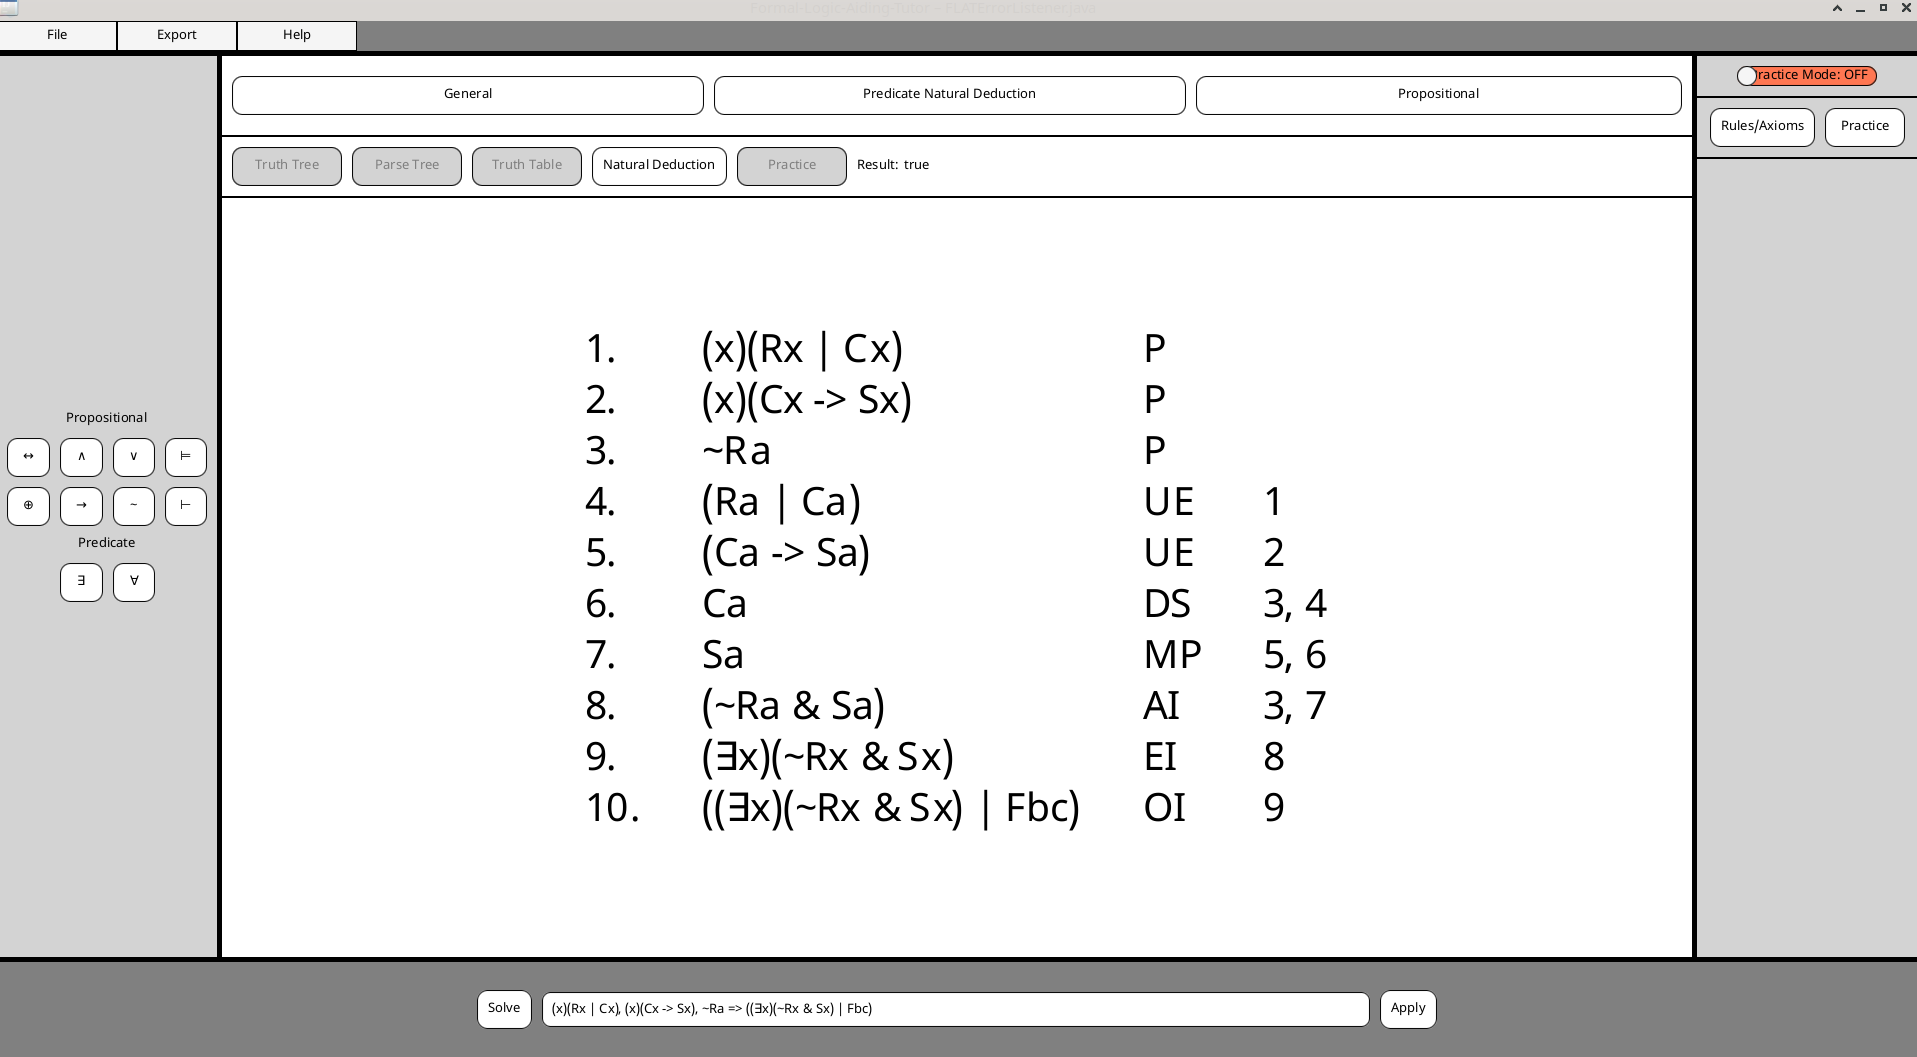
\includegraphics[width=0.9\linewidth]{flat1.png}
		\caption{Predicate Logic Proof}
		\label{fig:flat1}
	\end{subfigure}%
	\begin{subfigure}{.5\textwidth}
		\centering
		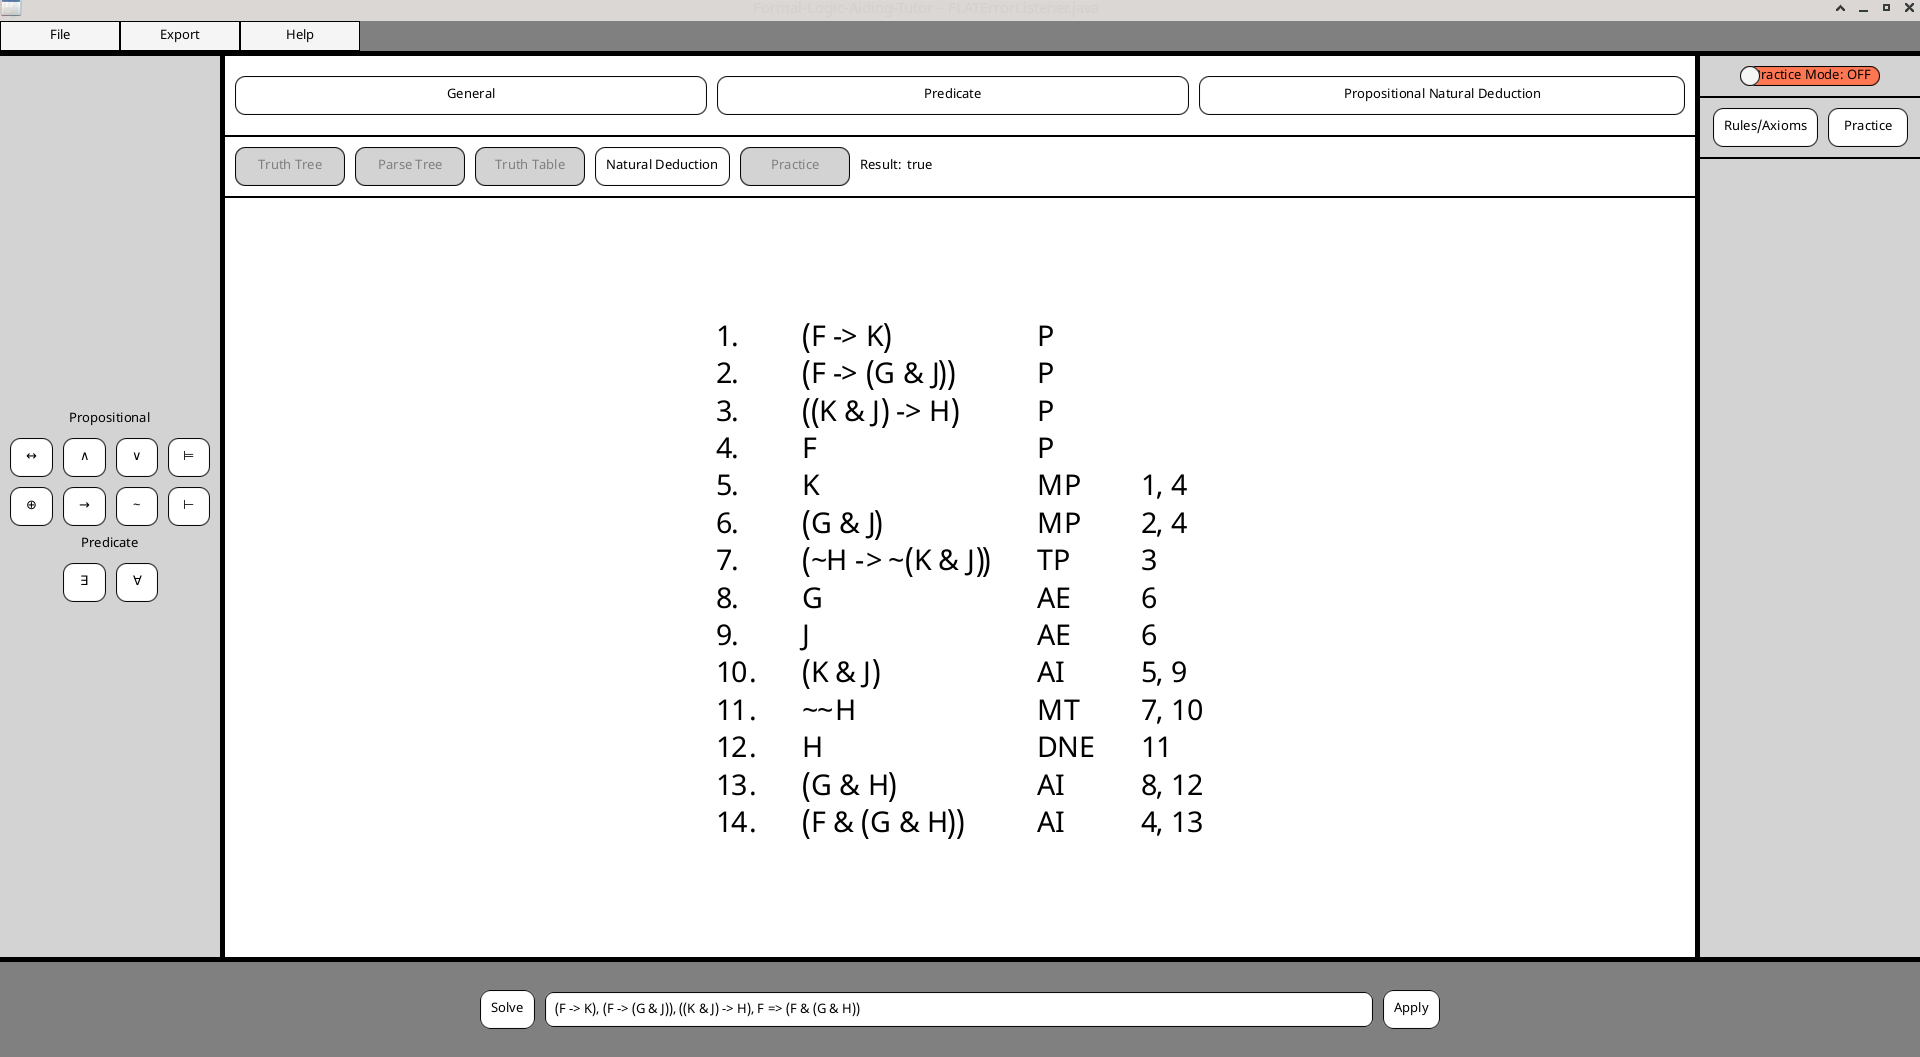
\includegraphics[width=0.9\linewidth]{flat2.png}
		\caption{Propositional Logic Proof}
		\label{fig:flat2}
	\end{subfigure}
	\caption{Two Natural Deduction Proofs Generated by FLAT}
	\label{fig:flatfigures}
\end{figure}

We will briefly explain some algorithms/subsystems, as well as other unique features of FLAT. For starters, students can export truth tables, truth trees (semantic tableaux) \cite{priest2008}, and natural deduction proofs as .pdf and .tex source files. This allows for easy submission and modification of, for instance, practice problems.

FLAT is translatable into a number of languages other than English via a Google Translate API to ease students into the world of the new language of formal logic without having to strictly learn English (note: this feature is highly experimentable and does not always produce optimal translations). 

Table \ref{table:flat} provides a list of a subset of the FLAT algorithms/subsystems that students can use to practice. Table \ref{table:flataxioms} shows the axiom base set for natural deduction proofs in FLAT.

\begin{table}
	\caption{Subset of Implemented Algorithms in FLAT}
	\label{table:flat}
	\small
	\begin{tabular}{p{3cm}p{11cm}}
	  \toprule
	  \thead{Algorithm}&\thead{Definition}\\
	  \midrule
	  Truth Tree&A truth tree is a description of the truth interpretations of a logic formula $F$.\\
	  Truth Table&A truth table is a sequence of true and false values evaluated for all models of a PL formula $F$.\\
	  Free Variable Detector&Finds all free variables in a FOPL formula $F$. An occurrence of a variable $v \in F$ is free iff there is no quantifier $Q$ that binds $v$ in its scope.\\
	  Bound Variable Detector&Finds all bound variables in a FOPL formula $F$. An occurrence of a variable $v \in F$ is bound if there is a quantifier $Q$ that binds $v$ in its scope.\\
	  Open Sentence Determiner&A FOPL formula $F$ is open if $\exists{v} \in F$ such that $v$ is free.\\
	  Closed Sentence Determiner&A FOPL formula $F$ is closed if $\forall{v} \in F$, $v$ is bound.\\
	  Ground Sentence Determiner&A FOPL formula $F$ is ground if $F$ does not contain any variables.\\
	  Main Operator Detector&A unary or binary connective $c$ is the main operator of a logic formula $F$ if it is the first-parsed operator when recursively evaluating $F$. If $F$ contains no connectives, then there is no main operator.\\
	  Vacuous Quantifier Detector&A quantifier $q$ in a FOPL formula $F$ is vacuous if it does not bind any variable $v$ in its scope.\\
	  Logical Tautology Determiner&A logic formula $F$ is a logical tautology if it is true in every interpretation/model.\\
	  Logical Falsehood Determiner&A logic formula $F$ is a logical falsehood if it is false in every interpretation/model.\\
	  Logical Contingency Determiner&A logic formula $F$ is a logical contingency if it is neither a logical tautology or logical falsehood.\\
	  Logically Consistent Determiner&Two logic formulas $F$, $F'$ are logically consistent if there a model $\mathcal{M}$ such that $F$ and $F'$ are true and $F_{\mathcal{M}} = F'_{\mathcal{M}}.$\\
	  Logically Contradictory Determiner&Two logic formulas $F$, $F'$ are logically contradictory if there is no model $\mathcal{M}$ such that $F_{\mathcal{M}} = F'_{\mathcal{M}}.$\\
	  Logically Contrary Determiner&Two logic formulas $F$, $F'$ are logically contrary if there is at least one model $\mathcal{M}$ that is false and $F_{\mathcal{M}} = F'_{\mathcal{M}}$, and there does not exist a model $\mathcal{M'}$ that is true and $F_{\mathcal{M'}} = F'_{\mathcal{M'}}$.\\
	  Logically Implied Determiner&Two logic formulas $F$, $F'$ are logically implied if there does not exist a model $\mathcal{M}$ such that $F_{\mathcal{M}}$ is true and $F'_{\mathcal{M}}$ is false.\\
	  Logically Equivalent Determiner&Two logic formulas $F$, $F'$ are logically equivalent if there does not exist a model $\mathcal{M}$ such that $F_{\mathcal{M}} \neq F'_{\mathcal{M}}$.\\
	\bottomrule
  \end{tabular}
\end{table}
\begin{table}[!ht]
	\caption{FLAT Natural Deduction Axioms}
	\label{table:flataxioms}
	\centering
	\begin{tabular}{lr}
	  	\toprule
	  	\thead{Axiom Name}&\thead{Definition}\\
	  	\midrule
	  	Modus Ponens (MP)&$(\phi \to \psi) \land \phi \therefore \psi$\\
	  	Modus Tollens (MT)&$(\phi \to \psi) \land \lnot{\psi} \therefore \lnot{\phi}$\\
	  	Hypothetical Syllogism (HS)&$(\phi \to \psi)\land(\psi \to \gamma)\therefore(\phi \to \gamma)$\\
	  	Disjunctive Syllogism (DS)&($(\phi \lor \psi) \land \lnot\phi \therefore \psi$\\
		Disjunction Introduction ($\lor${I})&$\phi \therefore (\phi \lor \psi)$\\
		Conjunction Elimination ($\land${E})&$(\phi \land \psi) \therefore \phi$\\
		Conjunction Introduction ($\land${I})&$\phi \land \psi \therefore (\phi \land \psi)$\\
		Material Implication (MI)&$(\phi \to \psi) \leftrightarrow (\lnot\phi \lor \psi)$\\
		Biconditional Breakdown (BCB)&$(\phi \leftrightarrow \psi) \therefore (\phi \to \psi) \land (\psi \to \phi)$\\
		Biconditional Introduction (BCI)&$(\phi \to \psi) \land (\psi \to \phi) \therefore (\phi \leftrightarrow \psi)$\\
		Double Negation Introduction (DNI)&$(\phi \therefore \lnot\lnot\phi)$\\
		Double Negation Elimination (DNE)&$(\lnot\lnot\phi \therefore \phi)$\\
		Transposition (TP)&$(\phi \to \psi) \leftrightarrow (\lnot\psi \to \lnot \phi)$\\
		Constructive Dilemma (CD)&$(\phi \lor \psi) \land (\phi \to \gamma) \land (\psi \to \omega) \therefore (\gamma \lor \omega)$\\
		Destructive Dilemma (DD)&$(\lnot\gamma \lor \lnot\omega) \land (\phi \to \gamma) \land (\psi \to \omega) \therefore (\lnot\phi \lor \lnot\psi)$\\
		DeMorgan's Law (DeM)&$\lnot(\phi \land \psi) \leftrightarrow (\lnot\phi \lor \lnot\psi)$\\
							&$\lnot(\phi \lor \psi) \leftrightarrow (\lnot\phi \land \lnot\psi)$\\
							&$\lnot(\phi \leftrightarrow \psi) \leftrightarrow \lnot((\phi \to \psi) \land (\psi \to \phi))$\\
							&$\lnot\exists\phi \leftrightarrow \forall\lnot\phi$\\
							&$\lnot\forall\phi \leftrightarrow \exists\lnot\phi$\\
		Existential Elimination ($\exists$E)&$\exists{x}Px \therefore P\alpha$ where $\alpha$ is not previously-used\\
		Existential Introduction ($\exists$I)&$P\alpha \therefore \exists{x}Px$\\
		Universal Elimination ($\forall$E)&$\forall{x}Px \therefore P\alpha$ where $\alpha$ is previously-used\\
	\bottomrule
  \end{tabular}
\end{table}

Like many existing systems, FLAT has its share of drawbacks. One of those is its tutoring system is rather primitive compared to others---while it has a ``tutoring mode" for almost all supported algorithms and subsystems, it does not generate exercises nor learn from an individual student's mistakes, which deems it non-intelligent according to the standard definition of an intelligent tutor \cite{woolf}. Also, there is no rhyme or reason why some first-order logic well-formed formulas infinitely loop whereas others do not (we suspect this is due in part to how it selects steps to complete a proof). Furthermore, the natural deduction system in FLAT is missing several key axioms e.g., commutativity and associativity as explained in section \ref{section:andtap}, which largely limits the set of solvable proofs. Moreover, when it cannot solve a proof, the system tries to perform a proof by contradiction, which sometimes leads it astray. We plan to drastically improve all features in future editions of FLAT.

\subsubsection{ANDTaP: Automatic Natural Deduction Tutor and Prover}\label{section:andtap}
ANDTaP is a smaller, web-based version of FLAT's natural deduction implementation. It supports a subset of its proving capabilities, but a superset of the tutoring functionality. Some natural deduction rules, e.g., associativity and commutativity, that are not present in FLAT work as intended in ANDTaP. The choice to use a web-based client for ANDTaP rather than a desktop application was highly influenced by the desire to allow students to use it wherever they want instead of being restricted to a locally-installed (desktop) program.

\begin{figure}[!ht]
	\centering
	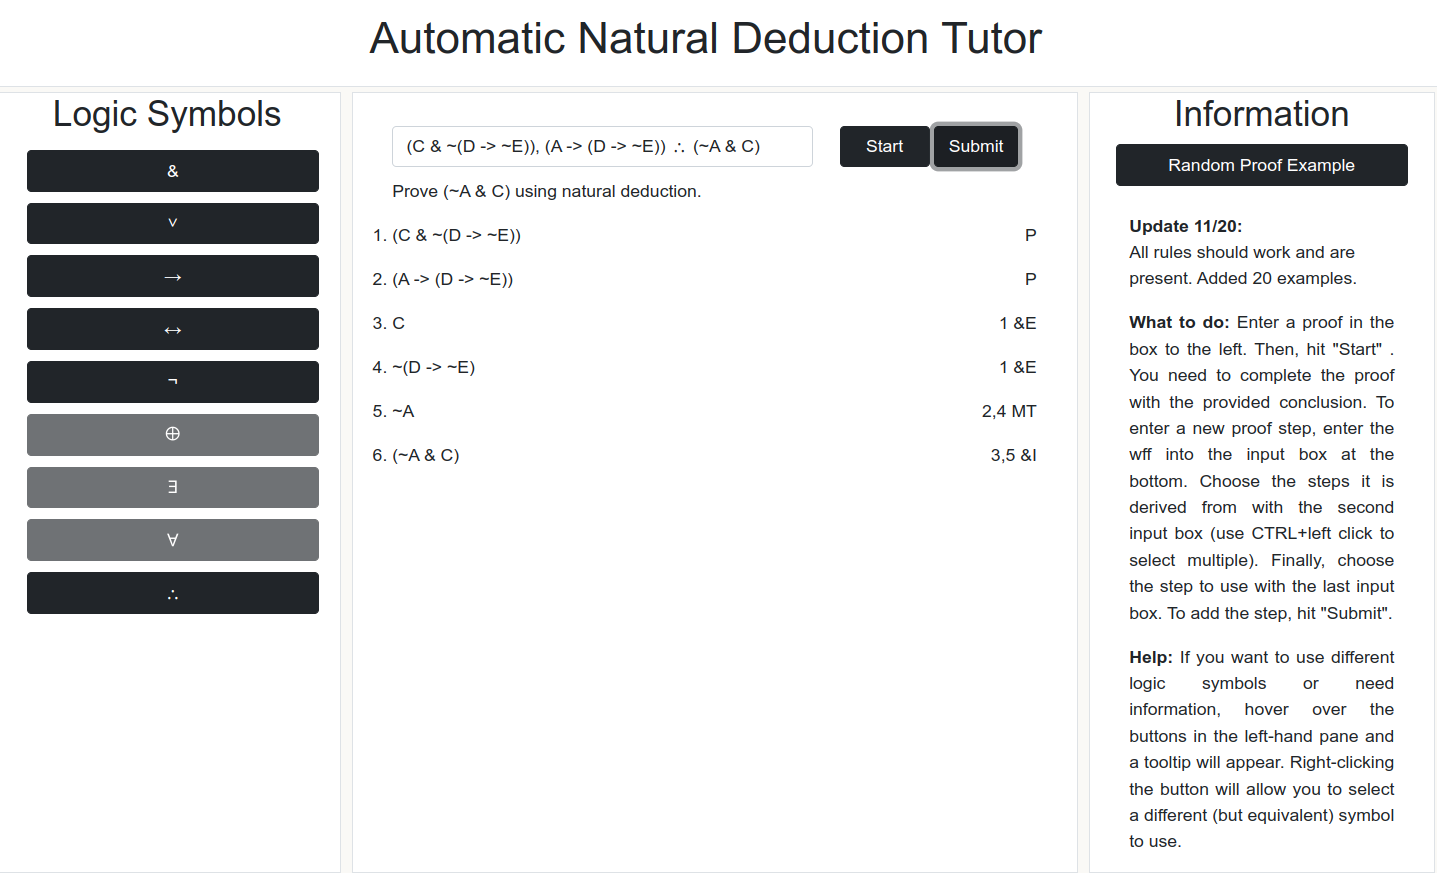
\includegraphics[width=0.9\textwidth]{andtap-tutor.png}
	\caption{ANDTaP Tutoring System}
	\label{fig:andtap}
\end{figure} 

Now that we have thoroughly discussed FLAT and ANDTaP, we will now explain, then discuss, the methods used to investigate several natural deduction systems in head-to-head comparisons against one another.

Systematically evaluating natural deduction software is complicated. For starters, as we previously mentioned, we still need a metric of analysis: how to directly compare one system to another. The best and systematic way to do this, excluding the possibility of a human study, is via the overall size of a proof (i.e., the number of lines a generated proof contains). Beginning students that receive a large and unwieldy result are likely to ignore its significance. Though, because the length of a proof does not report a conclusive answer to its complexity, we recorded the number of rules/axioms a system used compared to its base set size. The idea behind this decision is to provide insight into how often a system takes advantage of its axiom set, instead of trying to strictly use direct proofs (e.g., in Hilbert systems) or proofs by contradiction. 

We collected and created 288 well-formed formula propositional and first-order logic proofs from various logic and computer science textbooks \cite{lol} \cite{heinbook} \cite{methodsoflogic}. We manually converted each proof to the required syntax for all four system, then recorded the number of lines in the annotated proof as well as how many axioms/rules were used. Before we reveal and explain the results, we will briefly review each investigated system.

The first tool we analyzed was a web application for proving propositional logic natural deduction formulas by Laboratoire d'Informatique de Grenoble (LIGLAB) \cite{teachinglogic}. While their tool includes a few other argument verification tools (e.g., semantic tabuleaux solver for modal logic S4, a resolution prover for first-order logic), we focused only on its propositional logic proving ability. Users enter premises as a series of conjunctions followed by an implication to the conclusion. This syntax follows the standard proof idea which says if all premises are true, then the conclusion must be true (in other words, the premises logically imply the conclusion). Beginning students or those using an ever-so-slightly different notation may be frustrated to discover that they have to convert their entire input to this rigid standard to parse it correctly. Such restrictions mean that users must focus on formatting their input to what the system requires rather than what it outputs as a result. We did find that their prover solved every propositional logic proof in our suite, but we found that because the system has a small baseset of theorems/axioms, almost every proof is a proof by contradiction, resulting in several nested proofs which can be hard to decipher.
\begin{figure}[!ht]
	\centering
	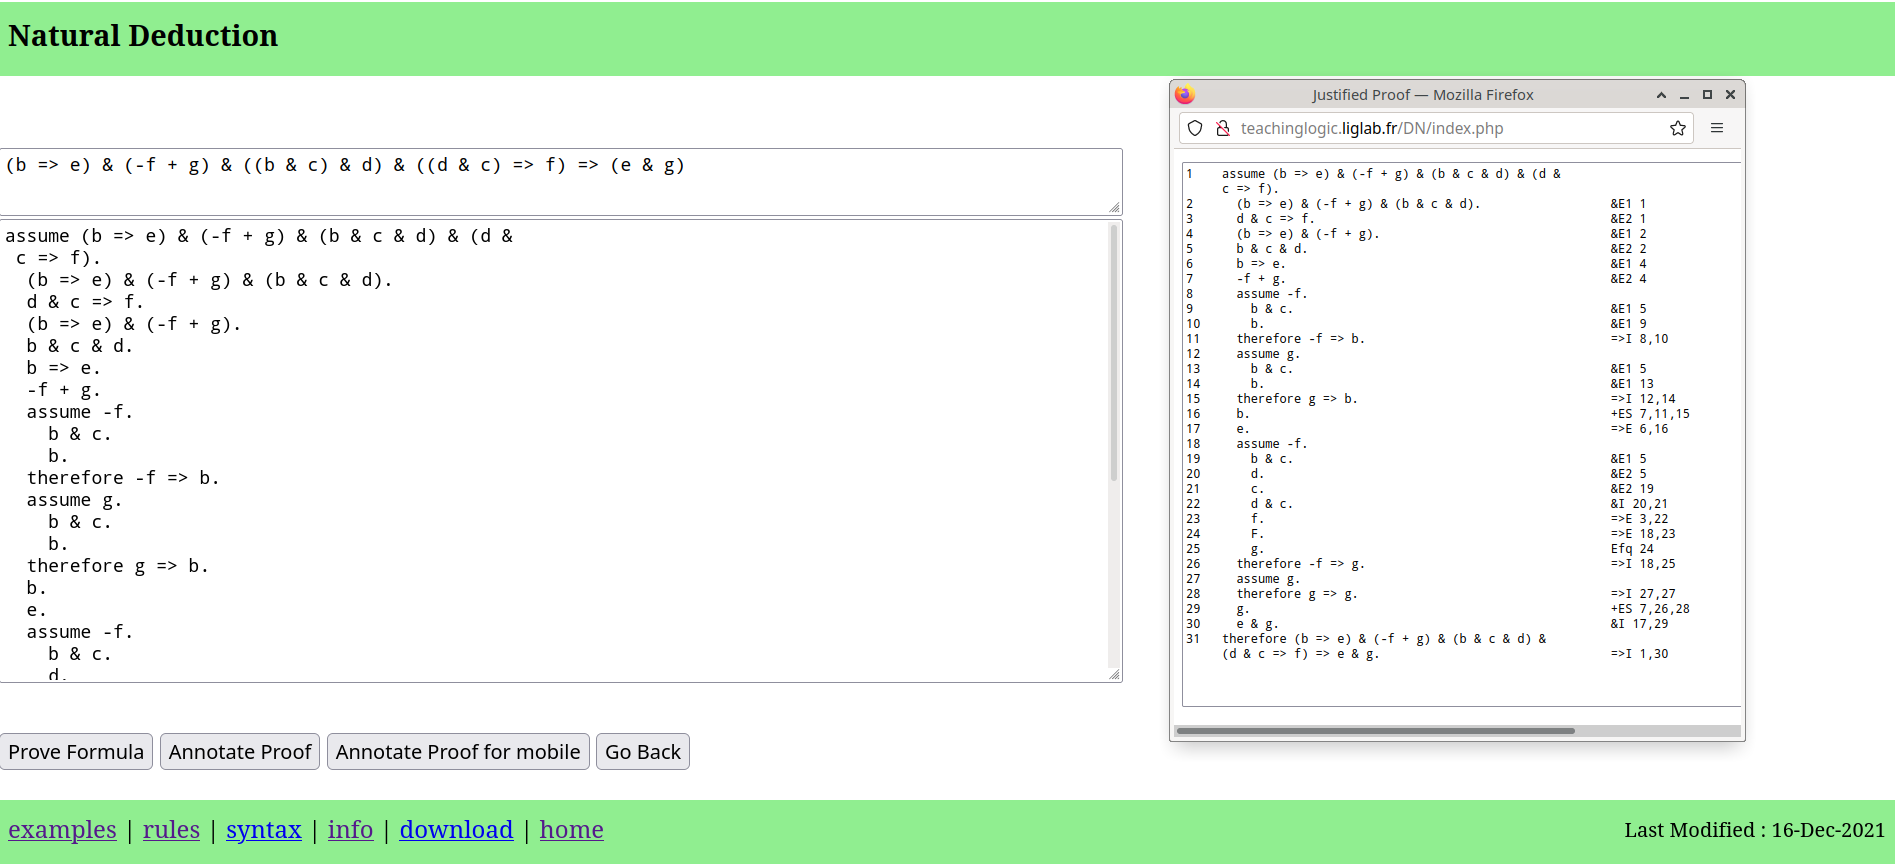
\includegraphics[width=0.65\textwidth]{teachinglogic.png}
	\caption{LIGLAB's Natural Deduction}{Example proof showing the user interface and proof annotations.}
	\label{fig:liglab}
\end{figure} 

Natural Deduction is a Windows 10 application designed by Jukka H\"akkinen, and is the second natural deduction software we investigated \cite{naturaldeduction}. This system includes both a proof generator and a proof checker. While it primarily focuses on modal logic (specifically, the modal logic system S5), it has a propositional logic prover because modal logic natural deduction semantics are a superset of those of propositional logic. We noted that its interface is clean and very elegant to use. Likewise, its ability to prove both theorems and premise-conclusion style proofs is helpful. We also found its performance on par, if not faster than other similar software. However, Natural Deduction has a severe drawback: its proof generation capabilities, or somewhat of a lack thereof. While it generates short and simple proofs for a subset of our test suite, for others, the proofs were unmanageably long and so cumbersome that a student would, realistically, never look through them. In addition to this significant issue, we discovered that the system places an arbitrary limit on the length of a premise set and its corresponding conclusion. Along a similar vein, the system refuses any proof that contains more than seven propositions/atoms, even if the proof contains no connectives - only atoms (e.g., $A$, $B$, $C$, $D$, $E$, $F$, $G$, $H$, $\therefore$ $H$). Lastly, the system automatically converts connectives to a recognizable format e.g., \textgreater\;to $\to$, and uppercases any entered propositions. It gets confused, though, if the user enters a symbol it does not recognize (e.g., \& instead of $\land$), and erroneously replaces symbols that otherwise together represent one into two separate symbols e.g., $=>$ into $\equiv\supset$. These restrictions do not entirely detract students from the application; however, they exemplify the types of downfalls that other systems do not have.
\begin{figure}[!ht]
	\centering
	\caption{NaturalDeduction Windows Application Solving a Proof}
	\label{fig:test}
	\begin{subfigure}{.5\textwidth}
		\centering
		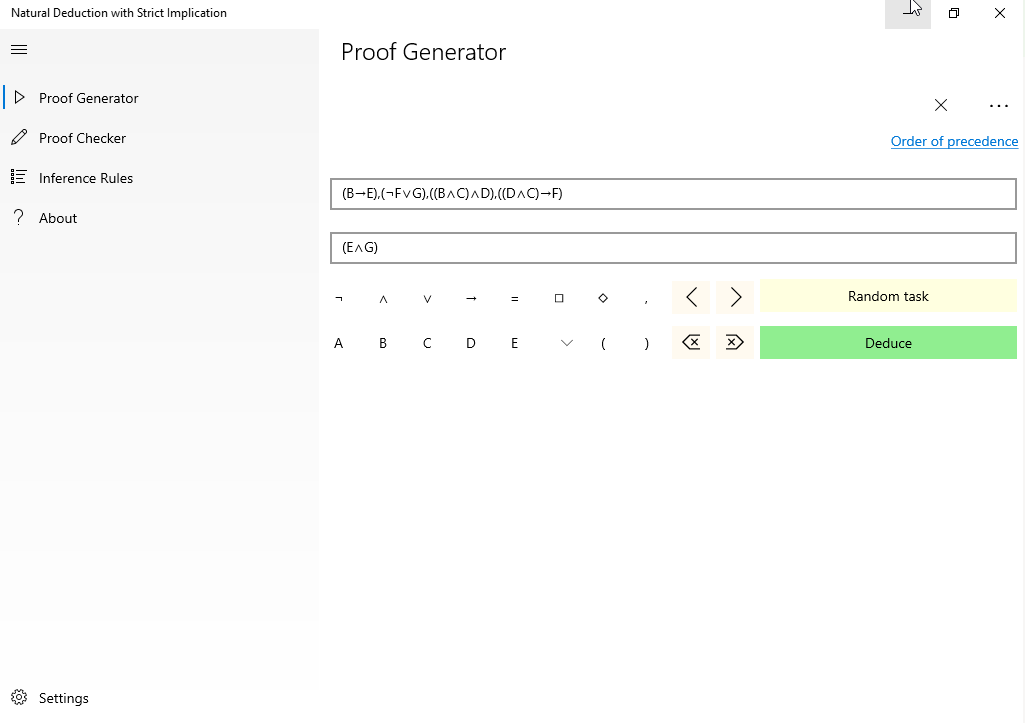
\includegraphics[width=0.9\linewidth]{w10app-1.png}
		\caption{Proof Input to System}
		\label{fig:sub1}
	\end{subfigure}%
	\begin{subfigure}{.5\textwidth}
		\centering
		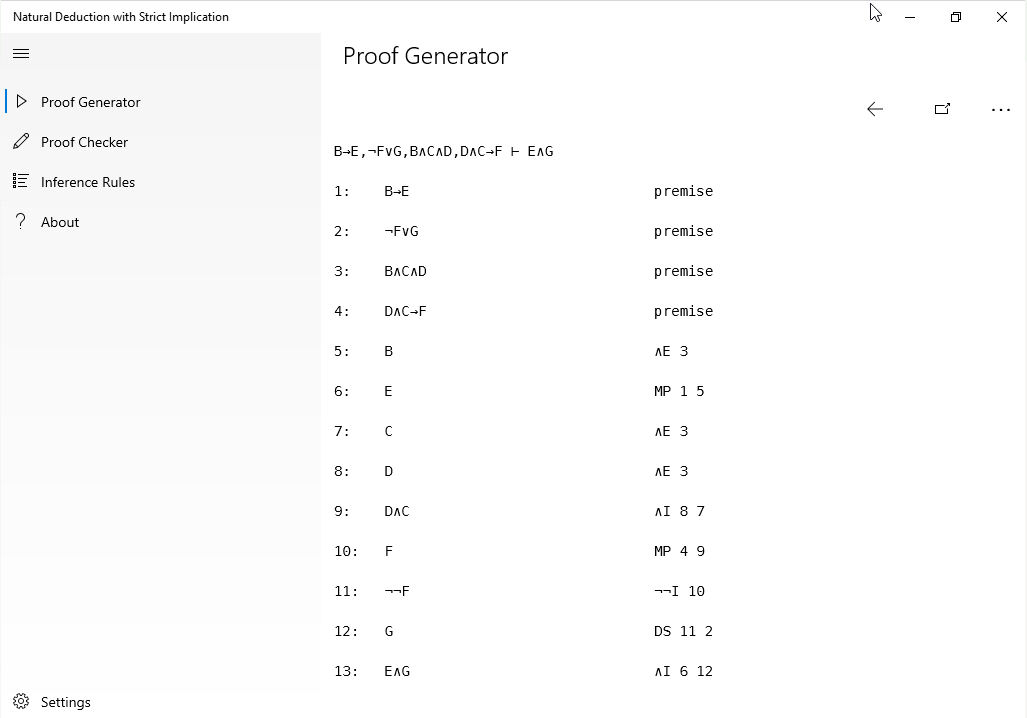
\includegraphics[width=0.9\linewidth]{w10app-2.png}
		\caption{Proof Output Solution with Annotations}
		\label{fig:sub2}
	\end{subfigure}
\end{figure}

TAUT-Logic is a web application designed by Ariel Roff\'e, and assisted by the Buenos Aires Logic Group \cite{taut}. Unlike the first two, TAUT-Logic supports first-order predicate logic, and is the only easy-to-use system of its kind that we found which is not out of commission nor abandoned. In addition to its natural deduction toolset, it supports basic set theory,  truth table generation, and model truth. 

One awkward characteristic of this system is that its propositional logic application only supports lowercase letters for atoms. Additionally, similar to Natural Deduction, TAUT-Logic supports a total of nine different atoms, ranging from $o$ to $w$. Supporting only nine atoms may be enough for some problems/proofs, but this restriction seems rather arbitrary for natural deduction, whose problem complexity should not grow strictly in terms of the number of atoms. Another odd design choice is the preference of English phrases for connectives instead of symbols such as, for example, ``implies'' versus $\to$ or $\supset$. Because all other systems we tested only utilize symbols (with the exception of FLAT, as it supports both), the process of converting each formula and symbol to the appropriate format was tiresome. Lastly, for some reason, the biconditional connective is not supported, requiring students to either convert them to a conjunction of implications, or omit the proof altogether. 
    
Regarding TAUT-Logic's performance, we discovered that it is roughly on par in terms of speed, but fails on moderately complex propositional and first-order logic proofs. We also saw a general increase in the produced proof size compared to the other systems. 
\begin{figure}[!ht]
	\centering
	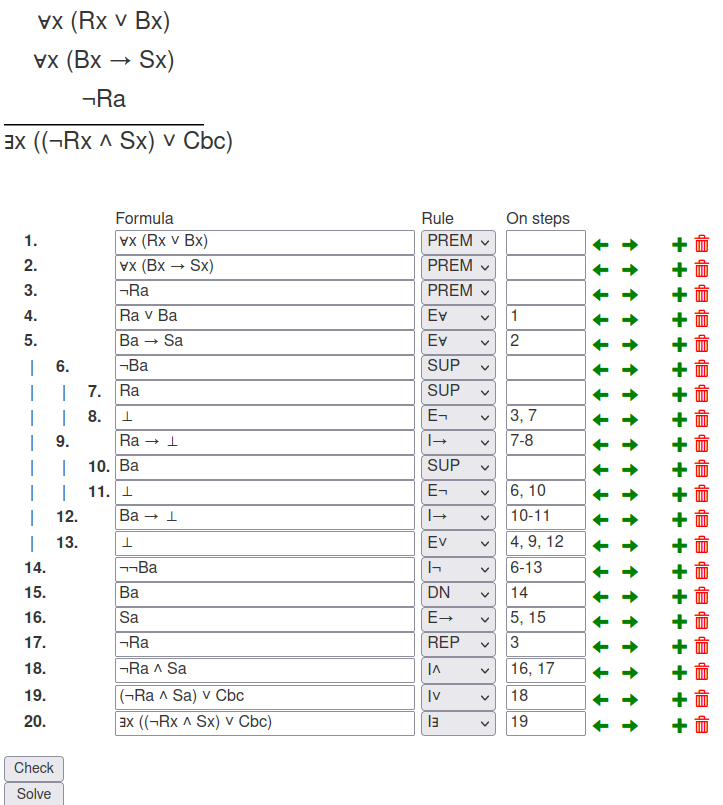
\includegraphics[width=0.4\textwidth]{tautlogic.png}
	\caption{TautLogic's Predicate Natural Deduction}{Write a caption...}
	\label{fig:tautlogic}
\end{figure} 

\subsubsection{System Comparison Results}
Table \ref{table:allData} shows the tabulated results, including the average number of applied distinct rules compared to the base set size, the average length of all proofs, and the average success rate. Note: systems that did not support first-order logic contributed to a lower overall success rate. Consequently, we further subdivided the data into two groups: one with only propositional logic formulas ($n=203$), and another with only predicate logic formulas ($n=85$). Also note that, when a system cannot solve a proof, this, in turn, lowers the average number of steps and applied distinct rules as those count as zero towards the average. Thus, we created another table to show non-zero total averages.
\begin{table}[!ht]
	\centering
	\caption{Data Analysis of Propositional and First-Order Logic Proofs}
	\begin{tabularx}{\textwidth}{*4c}
		\toprule
		System           & Avg. Success Rate & Avg. No. Steps & Avg. No. Distinct \\    
		\midrule
		\textbf{FLAT}    & \textbf{84.72\%}  & \textbf{5.86}  & \textbf{2.79}     \\
		TeachingLogic    & 70.49\%           & 12.41          & 3.77              \\
		NaturalDeduction & 56.60\%           & 13.50          & 3.38              \\
		TAUT-Logic       & 73.96\%           & 13.34          & 4.46              \\
		\bottomrule
	\end{tabularx}
	\label{table:allData}
\end{table}

\begin{table}[!ht]
	\centering
	\caption{Data Analysis of Propositional Logic Proofs}
	\begin{tabularx}{\textwidth}{*4c}
		\toprule
		System           & Avg. Success Rate & Avg. No. Steps & Avg. No. Distinct Rules \\    
		\midrule
		\textbf{FLAT}    & \textbf{85.22\%}  & \textbf{5.94}  & \textbf{2.67}           \\
		TeachingLogic    & 99.01\%           & 17.48          & 5.30                    \\
		NaturalDeduction & 79.31\%           & 19.03          & 4.73                    \\
		TAUT-Logic       & 76.35\%           & 15.59          & 4.71                    \\
		\bottomrule
	\end{tabularx}
	\label{table:propData}
\end{table}

\begin{table}[!ht]
	\centering
	\caption{Data Analysis of Predicate Logic Proofs}
	\begin{tabularx}{\textwidth}{*4c}
		\toprule
		System        & Avg. Success Rate & Avg. No. Steps & Avg. No. Distinct Rules \\    
		\midrule
		\textbf{FLAT} & \textbf{83.53\%}  & \textbf{5.62}  & \textbf{3.05}           \\
		TAUT-Logic    & 68.24\%           & 7.46           & 3.76                    \\
		\bottomrule
	\end{tabularx}
	\label{table:predData}
\end{table}

\begin{table}[!ht]
	\centering
	\caption{Non-Zero Data Analysis of All Proofs}
	\begin{tabularx}{\textwidth}{*4c}
		\toprule
		System           & Avg. No. Steps & Avg. No. Distinct Rules \\    
		\midrule
		\textbf{FLAT}    & \textbf{6.92}  & \textbf{3.30}           \\
		TeachingLogic    & 17.61          & 5.35                    \\
		NaturalDeduction & 23.85          & 5.96                    \\
		TAUT-Logic       & 18.04          & 6.03                    \\
		\bottomrule
	\end{tabularx}
	\label{table:nzAllData}
\end{table}
In chapter \ref{chapter:4} we will discuss the findings to our experiment, as well as the challenges we encountered when formatting and inputting the formulas from our dataset.

\section{Gold Standard for Formal Logic System Syntax}
There are several reasons why a standardized grammar does not necessarily already exist for formal logic. Firstly, symbol usage varies widely from one subject to the next. Case in point, notation used in computer science may contain subtle yet important differences from philosophy-esque logics. Secondly, preexisting sources such as textbooks, websites, professors, and others all use preferential notation (i.e., they use what they think is correct, what they were taught, or what is otherwise preferred in their respective discipline), providing an amalgamation of symbols for students to use and reference which, therefore, leads students and automatic systems astray when expecting one syntax yet receive something completely different. Thirdly, propositional logic learning platforms may or may not include certain operators. For example, because it is trivial to represent the biconditional (if and only if) binary operator as a conjunction of implications, it is certainly possible, albeit rather rare, to omit its symbolic representation from a language. Such omissions cause problems when evaluating formulas either automatically or by hand..... \textbf{continue here}

We propose a formal definition that aims to solve most of these problems. One component of this definition allows users to create their own logic language definition as they see fit for their situation. This language is then translatable into a gold standard format, which we will define syntactically and semantically.

\subsection{Zeroth-Order Logic Well-Formed Formula Representation}
We will start with a small example and then generalize the approach to achieve a well-defined representation. Suppose we have a set of premises $P = \{(A \leftrightarrow B),\,\lnot (C \land D),\,C,\,\lnot B\}$ with the conclusion $c = (\lnot A \land D)$. Converting this proof into the three systems we tested is laborious at best and is increasingly tiresome the more systems we wish to evaluate. Table \ref{table:requiredsyntax} displays the required syntax to parse an equivalent representation of $w$. The desire for a uniform standard to rapidly test multiple systems without manual intervention is readily apparent.
\begin{table}[!ht]
	\caption{Required Syntax to Parse Proof $(P,\,c)$}
	\label{table:requiredsyntax}
	\small
	\centering
	\begin{tabular}{lr}
	  \toprule
	  \thead{Natural Deduction System}&\thead{Syntax}\\
	  \midrule
	  TeachingLogic&$(p\,<=>\,q)\;\&\;\varlnot(r\,\&\,s)\;\&\;r\;\&\;\varlnot{q}\;=>\;(\varlnot{p}\,\&\,\varlnot{s})$\\
	  NaturalDeduction&$(A\,\equiv\,B),\,\lnot(C\,\land\,D),\,C,\,\lnot{B}\,\therefore\,(\lnot A \land \lnot D)$\\
	  TAUT-Logic&$(A\,\text{implies}\,B)\,\text{and}\,(B\,\text{implies}\,A),\,\text{not}(C\,\text{and}\,D),$\\
	  			&$C,\,\text{not}\,B\,\therefore\,(\text{not}\,A\,\text{and}\,\text{not}\,D)$\\
	\bottomrule
  \end{tabular}
\end{table}

Let $M(\mathcal{L},\,w)$ be a function that ``applies'' the zeroth-order logic language $\mathcal{L}$ to the well-formed formula $w$. Let $\mathcal{L}$ be a pair $(\delta,\,\zeta)$ where $delta$ is an connective mapping function, and $\zeta$ is an atomic literal mapping function. 

The bijective function $\delta$ maps two sets $\delta:\;X \to Y$, where $X$ is the set of input connectives defined by $\mathcal{L}$, and $Y \subseteq \{N,\,C,\,D,\,E,\,I,\,B,\,T,\,F\}$ is the set of output connectives defined by our grammar, where $|X| = |Y|$. Table \ref{table:zerothlogicconnectives} shows the meaning of each connective in $Y$. Note that the arity of any connective $\phi \in X$ must match the arity of its corresponding output connective $\psi \in Y$.
\begin{table}[!ht]
	\caption{Connective Symbols for Zeroth-Order Logic Gold Standard}
	\label{table:zerothlogicconnectives}
	\centering
	\begin{tabular}{lr}
	  \toprule
	  \thead{Semantic Meaning}&\thead{Connective Symbol}\\
	  \midrule
	  Logical Negation&$N$\\
	  Logical Conjunction&$C$\\
	  Logical (Inclusive) Disjunction&$D$\\
	  Logical Exclusive Disjunction&$E$\\
	  Logical Implication&$I$\\
	  Logical Biconditional&$B$\\
	  Logical Tautology&$T$\\
	  Logical Falsehood&$F$\\
	\bottomrule
  \end{tabular}
\end{table}

The bijective function $\zeta$ maps two sets $\zeta:\;A \to B$, where $A$ is the set of atomic literals $\phi \in A$ where $\phi$ is an atomic literal used in $w$, and $B$ is the set of output atomic formulas $a_{j}$ where $j \in [1,\,|A|]$.

We can now define the Polish (Łukasiewicz), or prefix notation grammar $G$ used to create a standardized notation for zeroth-order logic. This notation takes inspiration from Scheme-syntax with its parenthesization of connectives and operands. For this, we must extend the definition of typical Extended Backus-Naur Form to account for multiple-arity connectives. Thus, we introduce the notation \textless{$x$---R\textgreater} to indicate that $x$ is a variable used in the EBNF rule $R$, and $\{\gamma\}^{x}$ to denote $x$ applications of $\gamma$. In the grammar, $\alpha$ is the arity of a connective.
\begin{grammar}
	<atomic> ::= `a' (`1' | `2' | ...)
	        
	<connective> ::= `N' | `C' | `D' | `E' | `I' | `B' | `T' | `F' 
	        
	<$\alpha$---wff> ::= <atomic> | (<connective> [` '] \{<wff>\}$^{\alpha}$)
\end{grammar}
\subsubsection{Zeroth-Order Logic Example 1} Let us take a ``standard'' propositional logic language $\mathcal{L}$ and a formula $w$. $\mathcal{L}$ consists of two functions $\delta$ and $\zeta$ where
\begin{align*}
	  & \delta:\;\{\supset,\,\land,\,\lor,\,\leftrightarrow,\,\lnot\}\mapsto \{I,\,C,\,D,\,B,\,N\} \\
	  & \zeta:\;\{A,\,B,\,C\} \mapsto \{a_{1},\,a_{2},\,a_{3}\}                                   
\end{align*}
We will let $w = A \supset (B \leftrightarrow \lnot C)$. Thus, 
\[
	M(\mathcal{L},\,w) = (I\;a_{1}\;(B\;a_{2}\;(N\;a_{3})))
\]
This representation reads naturally from left-to-right as follows: ``An implication of $a_1$ and a biconditional of $a_2$ and negated $a_3$''. We consider all connectives as first-class functions in our definition.

While prefix notation is not as readable as the infix $w$, it creates a uniform standard for testing zeroth-order logic systems. What's more is that this application process is reversible; given $M^{-1}(\mathcal{L}',\,w')$ where $\mathcal{L}' = (\delta^{-1},\,\zeta^{-1})$ and $w' = M(\mathcal{L},\,w)$, we can reproduce $w$ using a simple stack-and-pop parsing evaluation approach (deterministic push-down automaton).
    
\subsubsection{Zeroth-Order Logic Example 2}
Quine's syntax in \cite{methodsoflogic} for propositional logic is slightly different from modern variants. Specifically, his use of dots and colons removes superfluous parentheses when defining operator precedence. Largely, we will ignore this notation in favor of his parenthesized form. In addition, Quine uses an empty string $\varepsilon$ to represent conjunction (e.g., $S_{1}S_{2}$ represents a conjunction between two well-formed formulas $S_{1}$ and $S_{2}$). Finally, negations on a single atom $p$ are condensed with a vertical overbar $\overline{p}$. To compensate for the digital representation, we will keep the negation in front of the atom (e.g., $-S_1$ where $S_1$ is a well-formed formula). Now, we define $\mathcal{L}$ with functions $\delta$ and $\zeta$ where
\begin{align*}
	& \delta:\;\{\supset,\,\varepsilon,\,\lor,\,\equiv,\,-\}\mapsto \{I,\,C,\,D,\,B,\,N\} \\
	& \zeta:\;\{p,\,q,\,r,\,s\} \mapsto \{a_{1},\,a_{2},\,a_{3},\,a_{4}\}  
\end{align*}
We will let $w = -((p\lor q)(-r\lor s)) \supset (-(p\lor q)s)$. Thus,
\begin{align*}
	M(\mathcal{L},\,w) =\;&(I\;(C\;(N\;(D\;a_1\;a_2))\;(D\;(N\;a_3)\;a_4))\\
					   	 &(C\;(N\;a_1\;a_2)\;a_4))
\end{align*}
This representation reads as ``An implication where the left-hand side is a conjunction between a negated disjunction of $a_1$ and $a_2$, and a disjunction of negated $a_3$ and $a_4$. The right-hand side of the implication is a conjunction between a negated disjunction of $a_1$ and $a_2$, and $a_4$.''

The reason we formalize the language definition is to allow different logic systems with varying syntax---some use lower-case atomic formulas, while others may restrict the alphabet to a subset. This definition allows different connective alphabets to map to the same symbol in the gold standard which provides a seamless translation to and from various host logic languages (i.e., the language of the implementing systems, assuming it does not, by default, use the gold standard internally). Another benefit of using prefix connective notation is its disambiguation of precedence. We assume the incoming formula is unambiguous according to its language grammar specification out of simplicity, but for completeness, we will define a precedence mapping function for the incoming formula $\Gamma$. By enforcing prefix notation in the gold standard, we no longer have to deal with the inherent complexities of operator precedence present in the commonly-used infix notation.

Let $\Gamma$ be an injective function that maps the set of connectives $\delta$ to $\mathbb{N}$, namely $\delta \mapsto \mathbb{N}$. $\Gamma$ is designed to give connectives in $\delta$ a priority level, where the closer its mapped natural number is to zero, the higher its priority. We define priority as the precedence of a connective. When a system defines $\Gamma$, it means that any ambiguous well-formed formula in its corresponding language is parsable without parenthesization. $\Gamma$, as an algorithm, automatically adds parentheses to disambiguate the formula... \textbf{continue here}

\subsubsection{Precedence Mapping Example} We will use the same functions $\delta$ and $\zeta$ from the first propositional logic example. We will also define $\Gamma$ as
\begin{align*}
	& \delta:\;\{\supset,\,\land,\,\lor,\,\leftrightarrow,\,\lnot\}\mapsto \{I,\,C,\,D,\,B,\,N\} \\
	& \zeta:\;\{A,\,B,\,C\} \mapsto \{a_{1},\,a_{2},\,a_{3}\} \\
	& \Gamma:\;\{\supset,\,\land,\,\lor,\,\leftrightarrow,\,\lnot\}\mapsto\{3,\,1,\,2,\,4,\,0\}                              
\end{align*}
Now, suppose $w = A \to \lnot B \to C \land \lnot A$. The precedence function parenthesizes/disambiguates $w$ to $((A \to \lnot B) \to (C \land \lnot A))$, which is then converted into the gold standard as
\[	
	M(\mathcal{L},\,w) =\;(I\;(I\;a_{1}\;(N\;a_{2}))\;(C\;a_{3}\;(N\;a_{1})))
\]
Since we consider $\Gamma$ to be optional (opting for a default precedence of logical negation, logical conjunction, logical disjunction, logical implication, then logical biconditional), a system without a defined $\Gamma$ should, optimally, output a warning when it parses an ambiguous well-formed formula. Defining $\Gamma$ allows for any ambiguous formula to be converted into one that is unambiguous, as we previously stated, and also allows for ``custom precedence'' levels (i.e., if we want to bind logical disjunction higher than logical conjunction, it is trivial to do so). Finally, some may question the associativity of connectives. We assume that all operators are left-associative, similar to traditional addition, subtraction, multiplication, and division. Though, it would be easy to define a separate associativity function similar to $\Gamma$.

\subsubsection{Natural Deduction Extension} It is simple to extend $G$ to support premises and conclusions using the same syntax. We can define a new function $N(\mathcal{L},\,P,\,c)$, where $\mathcal{L}$ is the same definition as before, $P$ is a set of well-formed formula acting as the premises of the proof, and $c$ is the well-formed formula acting as the conclusion of the proof. Our new grammar $G'$ is as follows:
\begin{grammar}
	<atomic> ::= `a' (`1' | `2' | ...)
	
	<connective> ::= `N' | `C' | `D' | `E' | `I' | `B' | `T' | `F' 
	
	<$\alpha$---wff> ::= <atomic> | (<connective> [` '] \{<wff>\}$^{\alpha}$)
	
	<premise> ::= (`P' <wff>)
	
	<conclusion> ::= (`H' <wff>)
	
	<proof> ::= (<conclusion> \{<premise>\})
\end{grammar}
The preceding grammar states that a premise is preceded by the letter $P$ standing for \textit{premise}, conclusions are preceded by $H$ for \textit{hence}, and a proof is a conclusion followed by zero or more premises (a proof with zero premises is a theorem).\\

\subsubsection{Natural Deduction Example}
Let's create a proof where $P = \{\lnot(C \lor D),\,D \leftrightarrow (E \lor F), \lnot A \supset (C \lor F)\}$, and $c = A$. We must redefine $\zeta$ in $\mathcal{L}$ as follows:
\[
	\zeta:\;\{A,\,C,\,D,\,E,\,F\} \mapsto \{a_1,\,a_2,\,a_3,\,a_4,\,a_5\}
\]
\noindent Therefore, 
\begin{align*}
	N(\mathcal{L},\,P,\,c) & = ((H\;a_1)\;                    \\
	                     & (P\;(N\;(D\;a_2\;a_3)))            \\
	                     & (P\;(B\;a_3\;(D\;a_4\;a_5)))       \\
	                     & (P\;(I\;(N\;a_1)\;(D\;a_2\;a_5))))
\end{align*}
We read this as ``Hence $a_1$ if $P_1$ is true and $P_2$ is true and $P_3$ is true'', where $P_1$, $P_2$, and $P_3$ are the individual premises that comprise the argument. This style largely resembles the way we write Prolog (conditional) rules. 

\subsection{First-Order Logic Well-Formed Formula Representation}
First-order logic is a superset of zeroth-order logic, meaning we can reuse most of our definitions from the previous section. We will, however, need to slightly redefine $\mathcal{L}$ to allow for mapping predicate definitions, constants, and variables. Further, so as to not confuse the function definitions from zeroth-order logic, we will instead use new letters to represent mapping functions unique to first-order logic semantics.

Let $\mathcal{L}$ be a quadruple $(\delta,\;\varsigma,\;\chi,\;\eta)$ where $\delta$ is a connective mapping function, $\varsigma$ is a predicate mapping function, $\chi$ is a constant mapping function, and $\eta$ is a variable mapping function. 

For first-order logic, we slightly modify $\delta$ from its zeroth-order definition in the sense that it now maps two sets $\delta:\;X \to Y$, where $X$ is the set of input connectives defined by $\mathcal{L}$, and $Y \subseteq \{N,\,C,\,D,\,E,\,I,\,B,\,T,\,F,\,Z,\,X,\,V\}$ is the set of output connectives defined by our grammar, where $|X| = |Y|$. $N$, $C$, $D$, $E$, $I$, $B$, $T$, and $F$ are identical in both syntactic and semantic meaning to zeroth-order logic as referenced in table \ref{table:zerothlogicconnectives}. Table \ref{table:firstlogicconnectives} shows the new operators added by first-order logic. Note that $Z$ and $X$ have arities dependent on the formula used, so we cannot restrict it syntactically. Identity $V$, on the other hand, is a binary operator.
\begin{table}[!ht]
	\caption{Connective Symbols for First-Order Logic Gold Standard}
	\label{table:firstlogicconnectives}
	\centering
	\begin{tabular}{lr}
	  \toprule
	  \thead{Semantic Meaning}&\thead{Connective Symbol}\\
	  \midrule
	  Universal Quantifier&$Z$\\
	  Existential Quantifier&$X$\\
	  Identity&$V$\\
	\bottomrule
  \end{tabular}
\end{table}

The bijective function $\varsigma$ maps two sets $\varsigma:\;A \to B$, where $A$ is the set of predicate letters $\phi \in A$ where $\phi$ is a predicate letter used in the wff $w$, and $B$ is the set of output predicate letters $L_{i}$ where $i \in [1, |A|]$.

The bijective function $\chi$ maps two sets $\chi:\;C \to D$, where $C$ is the set of constant letters $\psi \in C$ where $\psi$ is a constant identifier used in $w$, and $D$ is the set of output constant identifiers $c_{i}$ where $i \in [1, |C|]$.

Lastly, the bijective function $\eta$ maps two sets $\eta:\;E \to F$, where $E$ is the set of variable letters $\rho \in E$ where $\rho$ is a variable identifier used in $w$ and $F$ is the set of output variable identifiers $v_{i}$ where $i \in [1, |E|]$.

Now, similar to zeroth-order logic, we will construct the gold standard Polish notation grammar $\mathcal{M}$ for first-order logic. Likewise, we will utilize the previously-defined notation \textless{$x$---R\textgreater} to eliminate ambiguity with operator arity. Two points to note are that, because identity is a special connective in first-order logic, we restrict its syntactic definition to only constants and variables. Additionally, quantifiers have a restriction in that they must have at least one variable following their declaration, as well as a bound well-formed formula.
\begin{grammar}
	<constant> ::= `c' (`1' | `2' | ...)
	
	<variable> ::= `v' (`1' | `2' | ...)
	
	<literal> ::= <constant> | <variable>
	
	<predicate> ::= `L' (`1' | `2' | ...)
	
	<connective> ::= `N' | `C' | `D' | `E' | `I' | `B' | `T' | `F'
	
	<identity> ::= `V'
	
	<quantifier> ::= `Z' | `X'
	
	<$\alpha$---wff> ::= (<predicate> \{<literal>\}) \\| (<connective> [` '] <wff>$^{\alpha}$) \\| (<quantifier> <variable> \{<variable>\} <wff>)\\| (<identity> <literal> [` '] <literal>)
\end{grammar}
The above grammar states ...\textbf{continue here}

\subsubsection{First-Order Logic Example} We will, once again, use a ``standard'' first-order logic language $\mathcal{L}$ and a formula $w$. $\mathcal{L}$ has a quadruple of the four functions $\delta$, $\varsigma$, $\chi$, and $\eta$ where
\begin{align*}
	  & \delta:\;\{\supset,\,\land,\,\lor,\,\leftrightarrow,\,\lnot,\,\forall,\,\exists,\,=\}\mapsto \{I,\,C,\,D,\,B,\,N,\,Z,\,X,\,V\} \\
	  & \varsigma:\;\{P,\,Q,\,R\} \mapsto \{L_{1},\,L_{2},\,L_{3}\}                                                                       \\
	  & \chi:\;\{c,\,d\} \mapsto \{c_1,\,c_2\}                                                                                       \\
	  & \eta:\;\{x,\,y,\,z\} \mapsto \{v_1,\,v_2,\,v_3\}                                                                             
\end{align*}
Suppose $w = \forall{x}\forall{y}\lnot{Pxyc} \land (Qcd \lor \exists{z}Rz)$. Thus,
\begin{align*}
	\mathcal{M}(\mathcal{L},\,w) & = (C\;(Z\;v_1\;(Z\;v_2\;(N\;(L_1\;v_1\;v_2\;c_1)))) \\
	                   & (D\;(L_2\;c_1\;c_2)\;(X\;v_3\;(L_3\;v_3))))         
\end{align*}
We read this as ``A conjunction of a universal quantifier that binds $v_1$, a universal quantifier binding $v_2$, bound to the negation of $L_1\,v_1\,v_2\,c_1$ and a disjunction of the following: $L_2\,c_1\,c_2$ and an existential quantifier which binds $v_3$, bound to $L_3\,v_3$.''

\chapter{Discussion and Future Direction}\label{chapter:4}
In chapter \ref{chapter:3}, we detailed our methods of experimentation, including a survey-focused and student-driven methodology, a head-to-head comparison of publicly-available natural deduction proving software, and a gold standard syntax definition for both zeroth and first-order logics. In this chapter, we will discuss our general findings, and analyze future research potential.

\textbf{Describe the $n=2$ survey results...}

\textbf{Describe what we found from analyzing the ND software and why that led to a desire for a gold standard}
As Tables \ref{table:allData}, \ref{table:propData}, \ref{table:predData}, \ref{table:nzAllData}, and graphs \ref{fig:allproofsgraph}, \ref{fig:propgraph}, \ref{fig:predgraph} show, our system, FLAT, has a higher percentage of proofs that are what we consider digestable for a beginning logic student. It is desirable for a natural deduction proof to be understandable, comprehensible, and condensed enough where details are not omitted, but rather are fleshed out to provide a clear path to the solution. 

While TeachingLogic's system has a greater percentage of solved proofs than FLAT, NaturalDeduction, and TAUTLogic, we found its user interface to be unintuitive particularly when entering a formula with unrecognizable syntax according to their language grammar. This odd requirement strongly deters those who wish to use a natural deduction proving software, but perhaps focus more time modifying their input to fit the system specifications than that spent understanding the generated proof(s). Moreover, its limited axiom base set upper-bounds the kinds of proofs it can generate---resulting in several nested subproofs and proofs by contradiction. Importantly, the generated proofs are syntactically and semantically correct, but to someone with little prior experience in formal logic or mathematical proofs, it may come across as overwhelming. 

A severe problem with NaturalDeduction, as we previously mentioned, is its unnecessary inconsistency---the generated proofs range from perfect (in that they match the intended expert solution) to absolutely out of control nose dives into confusion. As an illustration, suppose we want to prove $P = \{(A \leftrightarrow B), (C \leftrightarrow B)\}$, $c = A\leftrightarrow C$. FLAT's solution, which we consider the optimal solution under our axiom set, has twelve lines including the premises and conclusion (see figure \ref{fig:long-ass-proof}). NaturalDeduction, on the contrary, has 247 lines. The absurd length we discovered is not exclusive to this proof; we found several other sets of premises and conclusions which caused the system to generate unimaginably long and incomprehensible proofs. Furthermore, its input requirements are unreasonably restrictive... \textbf{continue here}
\begin{figure}[!ht]
	\caption{Proof of $P = \{(A \leftrightarrow B), (C \leftrightarrow B)\}$, $c = A\leftrightarrow C$}
	\label{fig:long-ass-proof}
	\begin{center}
	\renewcommand*\linenumberstyle[1]{#1.}
		\begin{prooftree}
			{
			close with={\ensuremath{\ast}},
			}
			[(A \leftrightarrow B), just=P
				[(B \leftrightarrow C), just=P
					[(A \to B) \land (B \to A), just=\text{1 BCB} %3
						[A \to B, just=\text{3 $\land$E} %4
							[B \to A, just=\text{3 $\land$E} %5
								[(B \to C) \land (C \to B), just=\text{2 BCB} %6
									[B \to C, just=\text{6 $\land$E} %7
										[C \to B, just=\text{6 $\land$E} %8
											[A \to C, just=\text{4, 7 HS} %9
												[C \to A, just=\text{3, 8 HS} %10
													[(A \to C) \land (C \to A), just=\text{9, 10 $\land$I} %11
														[(A \leftrightarrow C), just=\text{11 BCI}] %12
													]
												]
											]
										]
									]
								]
							]
						]
					]
				]
			]
		\end{prooftree}
	\end{center}
\end{figure}

\textbf{Explain the gold standard and... why it's a good alternative to the current state-of-the-art?}

\bibliographystyle{acm}
\bibliography{myreferences}
\nocite{*}

%%------------------------------------------------------------------%%
%%------------------------- Appendices -----------------------------%%
%%------------------------------------------------------------------%%
%% If you choose not to have appendices, comment out the \appendix
%% line and the chapters below.
%%------------------------------------------------------------------%%
\appendix

\chapter{Propositional Logic Natural Deduction Algorithm}

This appendix describes the algorithm we used to find a natural deduction proof for propositional logic. The idea is to use a ``satisfiability'' algorithm (not to be confused with the Boolean satisfiability problem SAT... \textbf{is this needed? Probably not}). A wff $w$ is satisfied when it is used in the reduction or expansion of another well-formed formula $w'$. In essence, if $w$ is used to construct $w'$, then $w$ is satisfied. At a high level, we recursively compute goals for each premise, and if we can satisfy each goal, then the premise is satisfied. The procedure \textsc{Satisfy} uses rules for each axiom to determine if a premise can be either simplified or if, as a goal, it can be constructed using other premises. For example, suppose we have two premises $A$ and $B$ and we want to satisfy $A \land B$. \textsc{Satisfy} will recursively search through the well-formed formula (i.e., attempt to satisfy its operands from left-to-right) to determine if either have been previously satisfied. Given that $A$ and $B$ are already premises, and premises are, by default, satisfied, we can conlude that $A \land B$ is satisfiable. As another example, let us take the argument $P = \{A \supset (B \land \lnot C),\;\lnot (B \land \lnot C)\}$ and $c = \lnot A$. It is trivial to see that we can conclude $c$ from the premises in $P$ via a modus tollens rule. \textsc{Satisfy} works slightly different when this type of situation occurs. Because there is no way to individually solve intermediate formulas e.g., $B$, $\lnot C$, the algorithm searches for transformations and elimination rules e.g., modus ponens, modus tollens, disjunctive syllogism, transposition, material implication, etc., that may be applied to premises. In our provided example, we can apply modus tollens to the two premises and consequently satisfy $\lnot{A}$. $\lnot{A}$ is, therefore, added to $P$. The terminating condition is when $c$ is satisfied, or equivalently, $c \in P$. Because there are numerous transformations that may be applied to premises, we will omit their direct inclusion in favor of a broad description of behaviors. To prevent unnecessary premises, once a premise is satisfied, it can never be ``unsatisfied''. Moreover, if a premise was constructed, it cannot be redundantly destructed or vice versa. For instance, suppose we have premises $A$ and $B$. We can use a conjunction introduction $\land{I}$ rule to satisfy $A \land B$. The algorithm could, in theory, use a conjunction elimination $\land{E}$ rule to break $A \land B$ back down into its original components. Since such repeated applications blows up the size of $P$ (leading to a potentially infinitely long proof), we heuristically prevent its occurrence.

\begin{algorithm}
	\caption{Propositional Natural Deduction Satisfaction Algorithm}\label{euclid}
	\label{appendix:algorithm}
	\begin{algorithmic}[1]
		\Procedure{Prove}{$P,\;c$}\Comment{$P$ is a list of premises, $c$ is conclusion}
		\While{$c$ is not satisfied}
		\For{$i\gets{1}$ to $P$.length}
		\If{\textsc{Satisfy}($P[i]$)}
		\State $P[i].satisfied\gets{\textbf{true}}$
		\EndIf
		\EndFor
		\If{\textsc{Satisfy($c$)}}
		\State $c.satisfied\gets{\textbf{true}}$
		\EndIf
		\EndWhile
		\EndProcedure
	\end{algorithmic}
\end{algorithm}

We have described how the algorithm generates a proof, but there lies the issue that unnecessary premises may have been generated as part of the path to said proof. In other words, there may be steps that contributed to a later step, but ultimately do not contribute to the proof path which derived the conclusion, deeming them as superfluous steps. Each step in the proof has parent steps which generate the child. For example, if $A$ and $B$ are steps to generate $A \land B$, we denote $A$ and $B$ as its parent steps. These are used in a backwards path walk from the conclusion to find a solution to the proof. Note that there may be more than one solution to a proof; our algorithm simply picks the path which explores all parent steps until the original assumptions are reached. We denote an original assumption as the premises which were provided as part of the proof... \textbf{continue here. I may want to rewrite this later but the basic idea/structure is here}
\begin{figure}[!ht]
	\centering
	\begin{subfigure}{.5\textwidth}
		\centering
		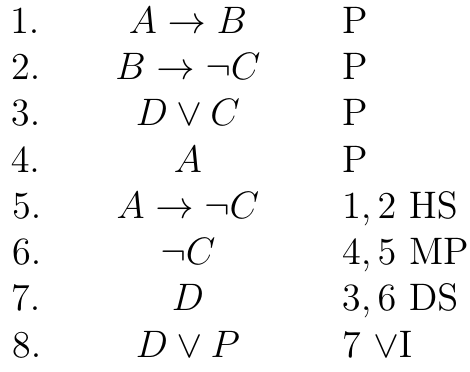
\includegraphics[width=.9\textwidth]{algorithmexample.png}
		\caption{Write a caption...}
		\label{fig:algorithmexample}
	\end{subfigure}%
	\begin{subfigure}{.5\textwidth}
		\centering
		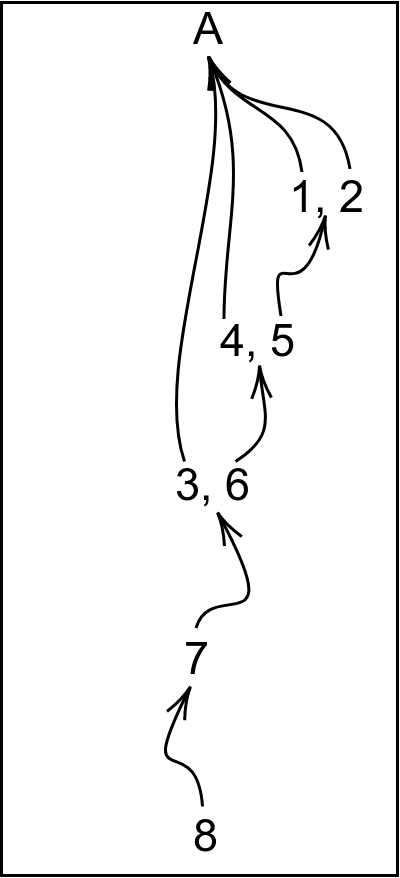
\includegraphics[width=.35\textwidth]{algorithmpath.png}
		\caption{Write a caption...}
		\label{fig:algorithmpath}
	\end{subfigure}
	\caption{Write a big caption!}
	\label{fig:togetheralgorithm}
\end{figure}

\chapter{Result Graphs}

\begin{sidewaysfigure}[ht]
	\centering
	
\includegraphics[width=1\textwidth]{all-proofs-graph.png}
	\caption{All Systems Natural Deduction Proof Line Count}
	\label{fig:allproofsgraph}
\end{sidewaysfigure} 

\begin{figure}[ht]
	\centering
	
\includegraphics[width=0.9\textwidth]{prop-graph.png}
	\caption{Propositional Logic Natural Deduction Line Count}
	\label{fig:propgraph}
\end{figure} 

\begin{figure}[ht]
	\centering
	
\includegraphics[width=0.9\textwidth]{pred-graph.png}
	\caption{Predicate Logic Line Count}
	\label{fig:predgraph}
\end{figure} 

\backmatter
\end{document}
